%------------------------------------------------------------------------------
% Template file for the submission of papers to IUCr journals in LaTeX2e
% using the iucr document class
% Copyright 1999-2013 International Union of Crystallography
% Version 1.6 (28 March 2013)
%------------------------------------------------------------------------------

\documentclass[preprint,pdf]{iucr}              % DO NOT DELETE THIS LINE

     %-------------------------------------------------------------------------
     % Information about journal to which submitted
     %-------------------------------------------------------------------------
     \journalcode{J}              % Indicate the journal to which submitted
                                  %   A - Acta Crystallographica Section A
                                  %   B - Acta Crystallographica Section B
                                  %   C - Acta Crystallographica Section C
                                  %   D - Acta Crystallographica Section D
                                  %   E - Acta Crystallographica Section E
                                  %   F - Acta Crystallographica Section F
                                  %   J - Journal of Applied Crystallography
                                  %   M - IUCrJ
                                  %   S - Journal of Synchrotron Radiation
%\usepackage[format=plain,justification=raggedright,singlelinecheck=false,font=small,labelfont=bf,labelsep=space]{caption}
%\usepackage{lineno}
\usepackage[pdftex]{graphicx}
%\usepackage{epstopdf}
\usepackage{float}

\begin{document}                  % DO NOT DELETE THIS LINE

     %-------------------------------------------------------------------------
     % The introductory (header) part of the paper
     %-------------------------------------------------------------------------

     % The title of the paper. Use \shorttitle to indicate an abbreviated title
     % for use in running heads (you will need to uncomment it).

\title{Online data analysis at ESRF BiosSaxs beam-line}
%\shorttitle{Short Title}

     % Authors' names and addresses. Use \cauthor for the main (contact) author.
     % Use \author for all other authors. Use \aff for authors' affiliations.
     % Use lower-case letters in square brackets to link authors to their
     % affiliations; if there is only one affiliation address, remove the [a].

\cauthor[a]{J\'er\^ome}{Kieffer}{jerome.kieffer@esrf.fr}{}
\author[b]{Adam}{Round}
\author[a]{Petra}{Pernot}
\author[a]{Martha}{Brennich}
\author[a]{Alejandro}{De Maria Antolinos}
\author[c]{Stefanie}{Hutin}
\author[a]{Guillaume}{Bonamis}
\aff[a]{ESRF, 71 avenue des Martyrs, 38043 Grenoble Cedex 9, \country{France}}
\aff[b]{EMBL Grenoble TODO \country{France}}
\aff[c]{UVHCI Grenoble\country{France}}

     % Use \shortauthor to indicate an abbreviated author list for use in
     % running heads (you will need to uncomment it).

\shortauthor{Kieffer et al.}

     % Use \vita if required to give biographical details (for authors of
     % invited review papers only). Uncomment it.

%\vita{Author's biography}

     % Keywords (required for Journal of Synchrotron Radiation only)
     % Use the \keyword macro for each word or phrase, e.g.
     % \keyword{X-ray diffraction}\keyword{muscle}

\keyword{Online data-analysis, solution scattering, protein}

     % PDB and NDB reference codes for structures referenced in the article and
     % deposited with the Protein Data Bank and Nucleic Acids Database (Acta
     % Crystallographica Section D). Repeat for each separate structure e.g
     % \PDBref[dethiobiotin synthetase]{1byi} \NDBref[d(G$_4$CGC$_4$)]{ad0002}

%\PDBref[optional name]{refcode}
%\NDBref[optional name]{refcode}

\maketitle                        % DO NOT DELETE THIS LINE

\begin{synopsis}
Low-latency data reduction and real-time feed back to the users
\end{synopsis}

\begin{abstract}
High throughput small-angle X-ray scattering on proteins in solution at
synchrotron sources is a commonly used technique in structural biology which
relies on highly automated data acquisition.
Data reduction and primary analysis for bioSAXS experiments consists of a
well-defined series of individual tasks whose automation allows easy first
assessment of the quality of collected data.
This article describes both the logic and the technical implementation of the
automated processing pipeline for bioSAXS data at the ESRF BM29 beam-line using
the EDNA framework.
\end{abstract}


\section{Introduction}
The popularity of small-angle X-ray scattering on proteins and nucleic acids in
solution (bioSAXS) to resolve their three-dimensional shape is continuously
growing \cite{Graewert2013,Hura2009,Reyes2014}.
This has not only resulted in the construction of new dedicated
synchrotron beam-lines, such as BM29 at ESRF, P12 at EMBL Hamburg or B21 at
Diamond Light Source \cite{BM29paper,P12,B21}, but also pushed forward new
developments in both beam-line instrumentation and sample handling.
<<<<<<< HEAD
Examples for these developments are the develoment of dedicated sample changers
=======
Examples for these developments are the new dedicated sample changers
>>>>>>> upstream/master
\cite{SCPaper} or the integration of size exclusion chromatography (SEC) systems
into existing beam-lines to ensure the monodispesity of the sample a a given
time \cite{SECPaper2012}.

The \textit{BioSaxs} beam-line, BM29, at synchrotron ESRF, is a small angle
X-ray scattering beam-line dedicated to structural biology \cite{BM29paper}.
Currently, the beam-line provides two main experimental modes: The use of the
bioSAXS sample changer to collect data on alternating buffer\/sample\/buffer
sequences (so called: sample changer mode) and an online HPLC system for
SEC-SAXS experiments (called HPLC mode).
In both modes, data are typically collected at a rate of one frame per second
(1 fps).
In order to estimate the quality and usefulness of the acquired data, it is
necessary process them in a quick and to robustly way, compatible with the
throughput of the beam-line.

Available processing tools for SAXS data which support online processing of
large data sets include \textit{DPDAK} \cite{DPDAK}, \textit{bioXTAS raw}
\cite{BioXTASraw}, \textit{SAXSutilities} \cite{SAXSUtilities} and
\textit{SASFLOW} \cite{X33P,P12},  \textit{XRDUA} \cite{XRDUA}, \textit{EDNA}
, \ldots 
Our goal is robust set of online autoprocessing pipelines
for bioSAXS data ranging from data reduction, primary analysis and \textit{ab
initio} modeling.
The additional needs of \textsc{flexibility} and elimination of
direct user interaction, lead us to develop a pipeline for both sample changer and HPLC mode within the
EDNA framework \cite{edna}.
These pipelines use pyFAI for the azimuthal integration \cite{pyFAI} and tools
from the \textsc{atsas} package \cite{ATSAS1, ATSAS2} for analysis and modeling.
Some parts of the \textsc{atsas} package have been re-implemented as a Python
<<<<<<< HEAD
library (named FreeSAS) for a better integration into the Python-based pipeline. 
All data analysis is smoothly integrated with the beamline control system
(BsxCube) and the ISPyB database.
=======
library (named FreeSAS \cite{freesas}) for a better integration into the
Python-based piepline.
All data analysis is smoothly integrated with the beam-line control system
(BsXCube) and the ISPyBB \cite{ISPYBB} database.
>>>>>>> upstream/master

\section{Technical background}

Online data analysis is a key component of any highly automated beam-lines
where the acquisition of a sample lasts for few seconds and there is
virtually no dead-time between samples.
Therefore the processing speed needs to keep up with the data acquisition, which
at ESRF-BM29 is typically one frame per second and about three minutes for a set
of background and sample measurements in sample changer mode.


\subsection{Experiment control}
Data acquisition at the ESRF-BM29 beam-line is controlled via the BsXCube
graphical interface, written in Python/Qt4 \cite{pyqt}.
BsXCube is composed of control-objects which communicate with other beam-line
components (i.e. detector, motors, sample changer, data analysis server\ldots)
via the tango protocol\cite{tango}.

%\subsection{Data analysis server}

%Data analysis is triggered automatically by BsxCube via a tango call.
%The data analysis server is actually a tango device server written in
%PyTango\cite{pytango} which launches EDNA jobs \cite{edna}.


\subsection{EDNA}
EDNA is a plugin-based framework to build pipelines for data-analysis.
The basic idea behind EDNA is to have plugins which are either responsible for the execution
of a task or an external process (called \textit{execution plugins}) or in
charge of launching and managing other plugins, either sequentially or in
parallel (called \textit{control plugins}).
The number of execution plugins running simultaneously is limited by processor
resources of the computer (and the Python global interpreter lock).
Any plugin receives its input arguments and returns its result using
data-structures (actually python objects) which can be serialized into XML for
sending them to disk or via the network.

An EDNA job is a top level control plugin which communicates with the outside
world, providing its state, or its results even after processing is finished,
while keeping its memory footprint as limited as possible.

\subsection{The Tango device server}
For accepting processing jobs from the outside, e.g. from the data
acquisition software (BsXCube), EDNA provides a Tango device server interface
\cite{tango,pytango}.
The device server starts EDNA jobs via the \textit{startJob} command.
The parameters of this command are a plugin name and the input data-structure
associated to it, and it returns a job identifier to the requester.
This tango device server is hence completely generic and can be used for any
type of EDNA jobs.

To have the best responsiveness at the tango level, EDNA jobs are not started as
they arrive but they are just instantiated and queued.
Another thread is responsible for starting them and can start multiple jobs in parallel
(data-parallelism). The number of jobs and the number of actual execution
plugins running simultaneously is controlled independently to do the best usage
of the computing power available within the single computer.

Once finished, any EDNA job emits a tango-event to announce the results are
available with the status: success or failure.
The data acquisition software, can then retrieve the result
of the processing, for example the 1D integrated scattering curve and
display it (without reading it from disk).
This architecture allows to start processing for individual images or
display curves instantaneously without polling the shared file-system.
Indeed, synchronization of shared file-systems across the network
often exhibits delay of multiple seconds.

\subsection{Hardware, software and versions}
Two computers with GP-GPU computing capabilities (Nvidia Quadro 4000) are
dedicated for online data analysis on the \textit{BioSaxs} beam-line, they are
independent and feature the same software installation.

As the \textit{ab initio} reconstruction pipeline lasts of dozens of minutes
(due to the execution of \textsc{dammin}, it is run on the most powerful
computer while the azimuthal integration pipeline, which needs the lowest latency, is run on
the small computer.
A third computer with similar computing capabilities is available for
off-line reprocessing, development of pipelines and acts as a spare.

All three computers are running Debian 7 operating system with \textsc{atsas}
(version 2.6.0).


\subsection{Preparation of protein sample and data acquisition}
 Move this section to Supplement??\\
All examples of protein data in this publication were acquired on the protein
D5TVE from Vaccinia virus (VACV).
The sequences of D5R is from the VACV strain Copenhagen (GenBank accession
number M35027.1). D5R 391-785 was cloned into the pProEx Htb (Invitrogen).
D5 was fused to an N-terminal hexahistidine tag that can be cleaved with the TEV
(tobacco etch virus) protease.
It was expressed in BL21* and purified over a (HIS-select; Sigma) (lysis buffer:
50 mM Tris pH 8.5, 150 mM NaCl, 5 mM MgCl2, Complete protease inhibitor cocktail
(Roche), DNase A, 10 mM beta-Mercaptoethanol; binding buffer: 50 mM Tris pH 8.5,
150 mM Nacl, 10 mM beta-Mercaptoethanol, High salt buffer: 50 mM Tris pH 8.5, 1
M Nacl, 10 mM beta-Mercaptoethanol, elution buffer: 50 mM Tris pH 8.5, 150 mM
Nacl,  200 mM imidazole, 10 mM beta-Mercaptoethanol).
The buffer of the eluates was exchanged to binding buffer on a PD10 column and
the protein was TEV-digested over night at RT.
The sample was injected onto a Superdex 200 GL 10/300 column (GE Healthcare)
equilibrated with gel filtration buffer (20 mM Tris pH 8.5, 150 mM NaCl, 1 mM dithiothreitol).
Eluted peaks were analyzed by SDS-PAGE and stained with InstantBlue (Expedeon).


\section{Data analysis pipeline in sample changer mode}

The sample changer allows a high throughput of different samples.
Before and after measuring a sample, a background measurement using its
corresponding buffer is performed.
If the buffer of a sample is the same as the one of the preceding sample, the
background measurement before the sample is dropped, as it is identical to the
buffer measurement after the preceding sample.
Hence, data is produced in sequences of the type \textit{buffer 1, sample 1,
buffer 1, buffer 2, sample 2, buffer 2, \ldots}  or  \textit{buffer 1, sample 1,
buffer 1,  sample 2, buffer 1 \ldots}.
Typically for each buffer or sample, 10 frames of 1~s exposure time are acquired.

The following steps for data reduction and analysis are required:
\begin{enumerate}
\item the integration of an individual frame,
\item the creation of a background corrected sample curve,
\item basic analysis of the sample curve (guinier plots, and other invariants)
\item \textit{ab-initio} modeling based on the basic analyis.
\end{enumerate}
In the EDNA bioSAXS application (ii) and (iii) are combined into one pipeline.

\subsection{Azimuthal integration pipeline}
\label{AI}
This pipeline is triggered for every single frame acquired, i.e. every second,
and therefore needs to have the lowest latency possible to display the integrated curve
in \textit{real time} in the graphical beam-line control interface BsxCube.
The input data-structure for azimuthal integration contains
information about the geometry of the experiment, the sample, its concentration
and the transmitted intensity (I1) as measured on the beam-stop diode for
normalization, etc.
To cope with the requested speed (up to 10 frames per second), this pipeline
has been optimized and simplified to the maximum.
It relies on the FabIO\cite{fabio} package for image reading (from NFS mounted disks) and
pyFAI\cite{pyFAI} for azimuthal integration.
As the images are acquired with a pixel detector (Pilatus 1M), the error can be
assumed to be Poissonian and is integrated as such.
The azimuthal integration calculation is performed on a dedicated graphics card
(Nvidia Quadro 4000) using OpenCL \cite{pyFAI_gpu}, offloading this processing
from CPU to GPU, hence leaving resources to other pipelines.
Subsequent normalization are performed directly using numpy\cite{numpy}.
The result is saved into a 3-column ASCII file suitable for further processing
using the \textsc{atsas} tools\cite{ATSAS1} and sent back to BsxCube for
live display.
In accordance with EMBL and ESRF standards, the scattering vector
$q=4\pi\frac{\sin(\theta)}{\lambda}$ is given in inverse nanometers.

\subsection{Curve merging, background correction and basic analysis}
\label{SM}
Data acquisition is usually performed sets of sample and buffer measurements.
Each sample or background measurment consists of seperate frames (typically 10)
in order to be able to detect radiation damage and not further interpret data from damaged samples.
The \textit{SmartMerge} pipeline is triggered at the end of each measurement
and is responsible for evaluating the similarity of different scattering
patterns, using the \textit{datcmp} tool from \textsc{atsas} and merging all frames
similar to the first and propagate the associated metadata.
A flow diagramm is provided in figure~\ref{fig:smart}.
All curve comparisons are performed in parallel on modern multicore
computers thanks to EDNA multi-threaded environment.

Subsequently, the \textit{SmartMerge} calls the \textit{autoSub} plugin, which
checks for the buffer-sample-buffer sequence and determines the optimal buffer
(see hereafter) and subtracts it from the sample data,  providing the so called
\textit{subtracted curve} containing only the scattering from the macromolecule.
If the buffer measured before and after the sample are considered sufficiently
similar by \textit{datcmp}, the optimal buffer is their average.
If they differ too much, each of them is subtracted individually from the
sample curve and the difference which results in the lower ratio of radius
of gyration $R_{G}$ over forward scattering intensity $I_{0}$, as determined by
the tool \textit{autorg} from \textsc{atsas} is retained.

(???)

If \textit{autorg} fails for both buffers, we simply use the one with the lower
total scattering. Figure~\ref{fig:autosub} provides a flow chart of the plugin.\\

Finally this \textit{subtracted curve} is analysed using the
\textit{SaxsAnalysis} plugin which performs subsequently uses tools from the \textsc{atsas} package for Guinier region fitting
using \textit{autorg}, Fourier transform using \textit{datgnom} to obtain
$p(r)$ and Porod volume assessement using \textit{datprorod}.
In addition the \textit{SaxsAnalysis} plugin creates \textit{PNG} figures of
the subtracted curve and the fit created by \textit{datgnom}, the Guinier fit, the $p(r)$ function and Kratky plots whenever possible (figure~\ref{plots}).
All these informations and figures are then directly returned to BsxCube to inform the user
of the success of the experiment and logged into the ISPyBB
database \cite{ispybb} where they can be accessed via an web interface.
Figure~\ref{fig:analysis} provides a flow chart of the plugin.

\subsection{Ab initio reconstruction pipeline}
\label{abinitio}
This pipeline is in charge of recontructing the three dimentionnal model based
of the \textit{subtracted curve} and is inspired from a preliminary work
performed at the Diamond Light Source \cite{DiamondSE}.

It runs multiple instances of \textit{dammif} in parallel (8 or 16 by default)
to get multiple models \cite{dammif}, taking benefit of the multithreading
environament of EDNA.
After a first round of outlier rejection based on the goodness of fit ($R_{f}$)
and the $\chi^{2}$  where the threshold is the mean plus a two standard
deviations, only $N$ valid models remains.

All $N$ remaining models are superimposed two by two using
our open source implementation of \textit{supcomb}, which is available freely
(MIT license)) as part of the freesas package \cite{freesas}.  
Former version of the pipeline have been using the original 
\textit{supcomb} \cite{supcomb} program from \textsc{atsas} by launching
$N*(N-1)/2$ processes in parallel within the EDNA framework. 
It turned out to be
more advantagous (in term of speed) to read all models from disk only once and
perform the all aligement in memory. 
Only distance calculation (actually normalized spatial discrepancy, NSD) have
been optimized using a binary extension (Cython parallel code), all other
transformation rely on NumPy \cite{numpy} code and the geomtric optimization is
performed using the simplex minimizer provided by SciPy \cite{scipy}.

The table containing the NSD is then generated
(see figure \ref{fgr:nsd}), explaining which model is the nearest from all other
valid models. This model is called the reference model and all other valid
models are re-oriented and aligned on the reference one. 
All models with a NSD higher than the mean plus one standard deviation are
discarded.

All valid models are merged using \textit{damaver}\cite{damaver},\textit{damstart} and
\textit{damfilt} and finally refined using \textit{dammin}\cite{dammin}.
This last step is pretty slow an lasts usually for dozens of minutes and is
aborted after half an hour by EDNA as it often does not finish. 
All results are uploaded to the ISPyB database where they can also be
visualized. Figure~\ref{fig:modeling} provides a flow chart of the plugin.


\section{Data analysis pipeline in HPLC mode}
While the sample changer allows a high throuput of samples, it requires
homogenous samples which do not degrade. 
Protein samples often are intrinsically heterogenous. 
For example, constituents of a complex might be present in excess or proteins
might aggregate.  
On approach to this issue is to purify the sample as shortly as possible before 
the measurement by directly collect data on the eluent a size exclusion system 
(SEC-SAXS or HPLC mode) \cite{SECPaper2012, otherSEC}. 
At the BioSaxs beam-line (BM29) we continously collect 2D-diffraction frames
throughout the SEC purification run at a rate of 0.5 to 1 Hz 
(depending on the synchrotron filling mode and the duration of the SEC purification), 
resulting in up to a few thousand frames. 
While we know that the first few frames are acquired on buffer, the sample composition 
for later frames is not known \textit{a priori}. 
The result of a SEC-SAXS experiement can be very complex. 
Our automatic analysis provides data reduction and basic analysis for every
individual frame. 
In addition, it uses this information to try to identify regions in the
chromatogram which correspond to one species and merges frames from these
regions for a better signal to noise ratio. 
The goal of this proceure is not to produce an idealized curve of an individual
species but to give a hint on the overall data quality as soon as possible.

\subsection{HPLC frame pipeline}

This pipeline is triggered for every frame in HPLC mode. 
It integrates each frame using the Azimuthal integration pipeline (see \ref{AI})
and compares the result to the first frame using \textit{datcmp} from the
\textsc{atsas} package. 
The frame is then classified as buffer, sample, or ``in between''. 
The first time a frame in a HPLC run is not classified as buffer, all previous
frames are averaged into a ``run buffer''. 
For any frame classified as sample, the ``run buffer'' is subtracted, Guinier
analysis is performed (with \textit{autorg} from the \textsc{atsas} package), 
providing a radius of gyration and the forward scattering intensity, and
correlated volume it calculated in order to estimate the mass
\cite{RamboTainerNature2013}. 
In addition, the plugin also calculates the total scattering intensity of any
frame, regardless of its classification.
The plugin can operate at about 1 Hz, so that the integrated frames can be
displayed in the data acquisition software with minimal delays. 
It also directly returns the total scattering intensity to the data acquistion
software so that it can display a chromatrogramm. 

Any frame very dissimilar to the first (using a second threshold) is considered
as a sample frame hence the averaged buffer signal is subtracted and Guinier
analysis is performed, providing a radius of giration and an intensity of
scattering at q=0. 

\subsection{HPLC flush}
When the HPLC experiment ends (or is aborted) a specific plugin is launched to
finish the processing of the experiment as one SEC-SAXS run. 
The plugin uses the results of \textit{autorg} to locate peaks using continous
wave transformation as implemented in Scipy on the forward scattering
\cite{cwt, scipy}, and then merges all individual curves around a local maxima
of the forward scattering with similar radius of gyration. 
All processing results from the \textit{HPLC frame pipline} and the results of 
the peak fiding are saved into a single HDF5 which is uploaded to the ISPyB
database at the end of the processing. 
In addition, the plugin creates figures (in .png and in .svg format) of the
total scattering, forward scattering and radius of gyration \textit{vs.} frame
number. 
Figure \ref{HPLC} shows the result of an HPLC experiment where one main peak and
a trailing shoulder is identified. 
On all merged files are further analysed by the \textit{SAXS analysis}
(\ref{SM}) and the \textit{Ab initio reconstruction pipeline}
(\ref{abinitio}) plugins from the sample changer pipeline.

\section{Offline data analysis}
In case offline processing is required, e.g. when when one of the parameters for
the azimutal integration of previsously processed data needs to be adjusted, 
several Python scripts for starting subpipelines are avaible. 
Those tools are part of the EDNA installation and just instanciate the needed
plugin and run it with the parameter description file which has been modified
accordingly. 
For HPLC mode and curve-merging, there are specific tools to reprocess complete
datasets if needed.

The drawback of this approach is to rely on the EDNA infrastructure which is
non trivial to install and even difficult to customize (path of the
\textsc{atsas} executable and licensing issue, number of cores, GPU
configration, timeouts for any part of pipelines, \ldots). 
The availability of a spare computer on the beam-line dedicated for offline
processing removes this need, hence reprocessing never interfers with ongoing
acquisitions.

\section{Practical example}
To illustrate the functionality of the processing pipeline we show data acquired
on a mutant of the helicase protein D5TVE from  of Vaccinia virus (VACV). 
Data was acquired as both a dilution series using the sample changer and using
SEC-SAXS.  
Results are shown in figures \ref{fig:HPLC} and \ref{fig:exp}. 
The HPLC run shows a strong main peak with extended tails both sides. 
Direct comparison of the different concentrations from the dilution series only
shows differences at very small $q$ (figure \ref{fig:exp}a)), but direct comparison 
of the highest concentration to the merged data from the main peak from the HPLC run 
shows only small differences (figure \ref{fig:exp}b).
The automatic processing results, especially the trends in $R_{G}$  clearly show the 
presence of concentration effects in the samples measured with the sample changer. 
In this particular case it is clear that the quality of the data collected with SEC-SAXS 
are of superior quality and that only they should be considered for further
processing.

\section{Conclusion}

TODO

\section{Conclusions and Outlook}
offline processing interface, workflows

\ack{The authors would like to thank Ricardo Fernandes and Thomas Boeglin for
developing the original offline reprocessing tools, Peter Boesecke for the
original azimuthal integration procedure, Olof Svensson for the development of
EDNA, Irakli Sikharulidze for the original version of the \textit{ab initio}
modeling pipeline, Alexey Kikhney, Daniel Franke and Dmitry Svergun for the
\textsc{atsas} package and support in its implementation and Staffan Ohlsson and Matias
Guijarro for integration with the data acquisition software.}

\bibliographystyle{iucr}
\bibliography{biblio}

\appendix
\section{Software distribution and licensing}

All software developed for online data analysis at the BioSaxs beam-line is
open-source.
Nevertheless it relies on the \textsc{atsas} package which, while free for
academic use, is neither open-source, nor redistributable.

EDNA is licensed under LGPL for the kernel part (the pipeline engine) and GPL
for the BioSaxs part. The source code is now hosted on a public
repository at https://github.com/edna-site. While open-source, EDNA is a
server tool for online data analysis and the developers are aware how difficult
it may be to install and configure it properly. EDNA is controling
\textsc{atsas} modules by executing external programs in pipe-mode to avoid any
licencing issues.

The azimuthal integration is performed via pyFAI\cite{pyfai}, the Python library
for fast azimuthal integration, which is accelerated on GPU\cite{pyfai_gpu}.
Diffraction image reading is performed by FabIO \cite{fabio}.
Both libraries
are licensed under GPL and hosted under those web pages:
http://github.com/pyFAI and https://fable.sf.net.
Some \textsc{atsas} parts have been implemented in Python to offer a better
integration into the processing pipelines (by avoiding the fork of many
processes): \textit{dataver}, \textit{damaver}, \ldots  and \textit{supcomb}
are available as part of the FreeSAS package which re-implements the
algorithms in a MIT type license. Freesas is available on github at
https://github.com/kif/freesas but without garanteeing any
numerical equivalence with the reference implementation.

Finally the other tools of the Python scientific stack (Numpy, scipy,
matplotlib) are licensed under BSD license.

\begin{figure}
\centering
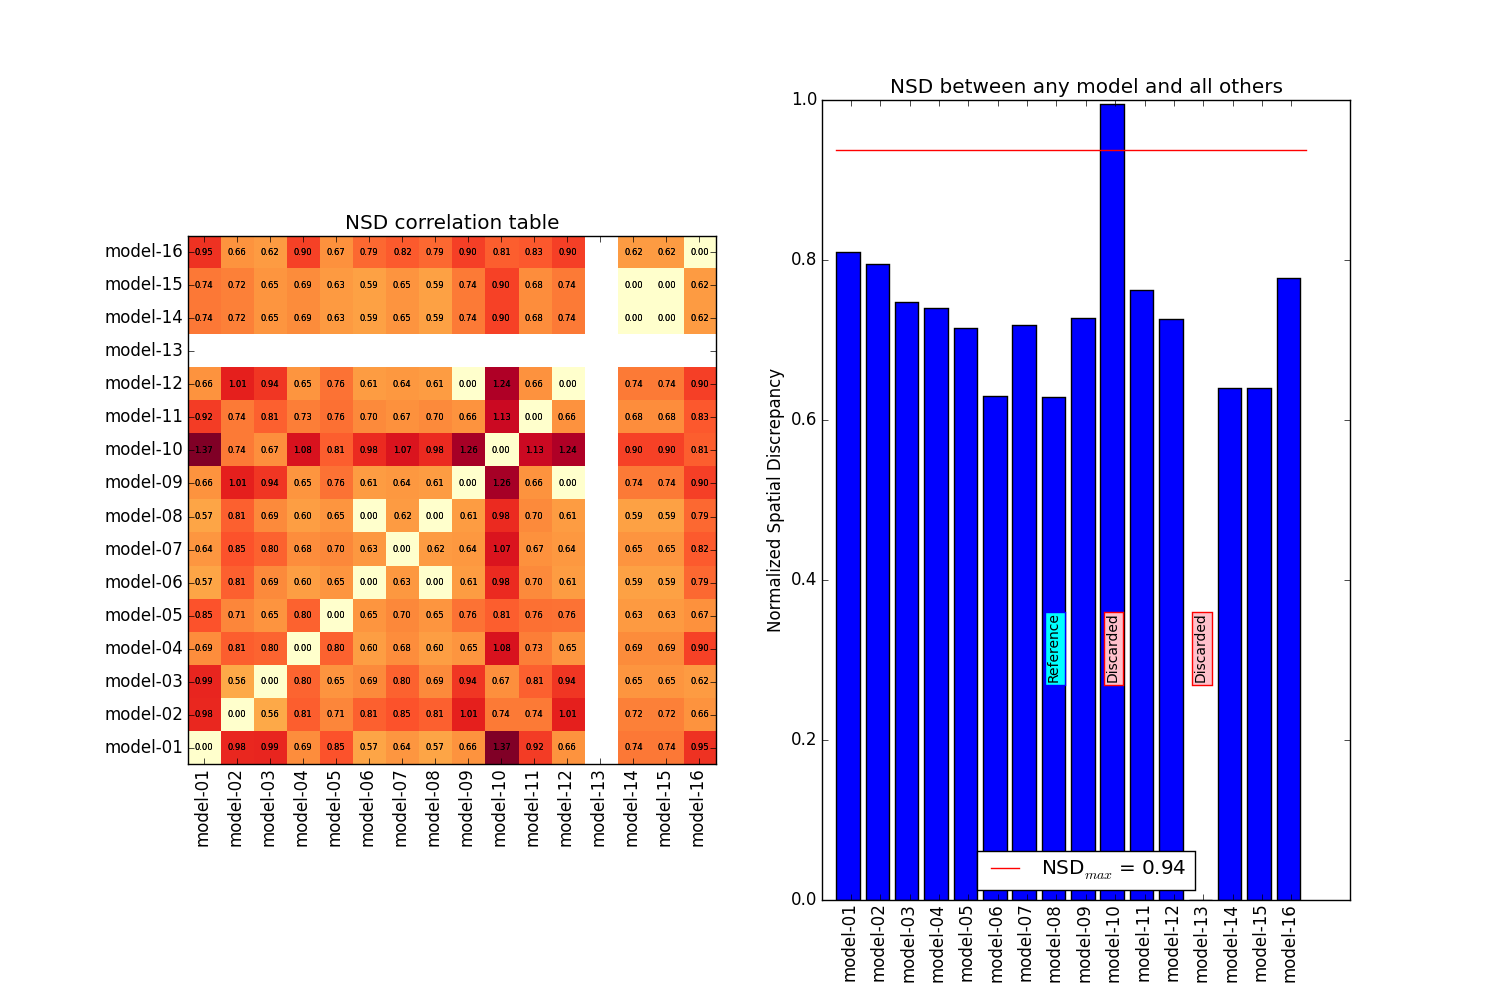
\includegraphics[width=8cm]{nsd.png}%
\caption{Plots created by the pipeline for comparing a set of \textit{ab initio} models. The matrix on the left hand site gives the pair-wise normalized spatial discrepancy (NSD) between two models. Thebar plot on the right hand site gives the mean NSD. The layout is adjusted from the standard verion for improved readability in print.}
\label{fgr:nsd}
\end{figure}

\begin{table}
\begin{tabular}{ l c | c c c c c c }
   & $c$  & $I_{0}$  & $R_{G}$ & $D_{max}$ & $V_{P}$ & $V_{c}$ & Mass from $V_{c}$\\
	 &  (mg/ml) & (kDa) & (nm)&  (nm)&  (nm$^{3}$) & (nm$^{2}$) & (kDa)\\
\hline
Sample changer & 5.00  & 35.06 & 2.80 & 9.37  & 72.00 n& &  \\
Sample changer & 2.50  & 34.28 & 2.83  & 9.91  & 72.08 & &  \\
Sample changer & 1.25 & 33.58& 2.86  & 8.74  & 69.82 & &  \\
Sample changer & 0.62  & 35.1& 2.99  & 10.48 & 73.89 & &  \\
Sample changer & 0.31 & 35.83  & 3.26  & 8.72  & 74.42& &  \\
HPLC, top of peak & - & 183.16 & 2.72  & -  & - & 4.08 & 49.70 \\
HPLC, merge & - & 123.89 & 2.70  & 9.46 & 69.97 & &  \\
Manual merge & - &  149.90 & 2.69 & 8.25 & & &  \\
\end{tabular}
\caption{Overview on the automatic processing results }
\label{tbl:results}
\end{table}


\end{document}
